\chapter{Evaluation}
\label{chap:evaluation}
In this chapter, our objective is to assess and examine the existing search engine implementation. The evaluation process is structured into three primary segments: Crawler, Indexer, and User Experience.

\section{Testing Environment}
The evaluation procedure is significantly influenced by the specific computing device executing the tests. Displaying information about the testing machine utilized can provide enhanced clarity and facilitate meaningful comparisons.


\begin{table}[ht] 
{\footnotesize
\begin{tabular}{ P{2.5cm} ||P{11.1cm}  }      % centered columns (3 columns) 
 \hline \hline
\textbf{Operating System} & Ubuntu 22.04.3 LTS \T\B 
\\ 
\hline
\textbf{CPU} & Intel(R) Core(TM) i7-10510U @ 1.80GHz; 4 cores; 8 threads \T\B 
\\ 
\hline
\textbf{RAM} & 32GB\T\B 
\\ 
\hline
\textbf{Machine} & Lenovo ThinkPad P15s Gen 1\T\B 
\\ 
\hline \hline
    \end{tabular}
}
  \captionsetup{justification=centering,margin=2cm}
  \caption{Local machine setup}
\end{table}

\section{Crawler}  

To evaluate the web crawler, the following criteria can be employed for measurement:


{\renewcommand\labelitemi{}
\begin{itemize}
  \item \textbf{Coverage}: This metric measures the proportion of relevant web pages that the crawler can locate and fetch from the internet.

  \item \textbf{Scalability}: It evaluates the crawler's facility for efficiently scaling up to add more computing power to crawl more content.

  \item \textbf{Versatility}: Can the crawler be applied to explore diverse types of content from various websites, encompassing text, multimedia, and links?

  \item \textbf{Robustness}: The crawler's ability to adeptly manage challenging scenarios and errors.

  \item \textbf{Politeness}:  the extent to which the crawler respects the rules and policies of the web servers and avoids overloading them with requests and forbidden links.

\end{itemize}

\subsection{Datasets} 
Evaluating a web crawler necessitates the utilization of a static website as a reliable reference point. The crawler-test\footnote{\url{https://crawler-test.com/}} website serves as an excellent choice for this purpose due to its diverse range of content and links, containing a wide range of scenarios that a crawler might encounter. This website effectively employs robots.txt to provide guidance to the crawler, allowing for an assessment of its politeness. Moreover, it includes a section containing links that yield various HTTP request status codes, such as 4xx and 5xx, which proves valuable for ensuring the crawler's robustness. Additionally, it incorporates multiple instances of page redirection, including scenarios like infinite redirection, which serves the dual purpose of evaluating the crawler's ability to avoid traps and enhancing its overall resilience.

To enhance the coverage and versatility of our crawler testing, we are considering two additional websites encompassing a broader range of use cases, ensuring that the crawler can effectively handle various HTML structures and more generic scenarios.
The first use case involves extracting product information from an E-commerce platform like Douglas\footnote{\url{https://www.douglas.de/}}. This website offers over 160,000 diverse products, making it an ideal candidate for testing different content types, including images. We will categorize our testing into three distinct datasets: small (with 100 products), medium (with 1,000 products), and large (with 10,000 products) to evaluate the crawler's performance under different data sizes thoroughly.
The second website, Times Higher Education\footnote{\url{https://www.timeshighereducation.com/world-university-rankings/2023/world-ranking}}, specializes in annually ranking universities. This unique characteristic allows us to evaluate content changes occurring on a yearly basis, setting it apart from other websites that undergo daily alterations, which can prove challenging for accurate evaluation.

\subsection{Experiments}
The crawler-test website is selected to assess and experiment with various crawler configurations. This choice is attributed to its stable, non-changing nature, which facilitates straightforward and meaningful comparisons of results across different configurations.
 
The first testing case is the coverage. It is vital to ensure the crawler can find the links inside the page, navigate to them and crawl them. 

Table \ref{table:crawler_test_config} displays the testing configurations used in the experiment. The Seed URL serves as the initial point from which the crawler begins its procedure, set to the root path of the crawler-test. The "Allow Multi Elements" checkbox is disabled (set to False) because the objective is not to gather a list of documents; each page contains a single text field. The Max Pages parameter is configured to a limit of 500, ensuring that the crawler does not exceed this number of pages. This figure can be adjusted based on the website's size to be crawled; for instance, smaller websites with around 50 pages may require a lower limit. The number of threads is set to the default value of 1.
We have set the Max Depth to 1 to enable easier coverage testing. This choice allows for easier comparison between the number of visited pages and the number of URLs discovered in the site's root path, which, upon simple page inspection, contains 415 links. Since the expected maximum number of pages is 415, the Max Docs parameter can be constrained to 500.
The inspectors are set to target the content of each page; thus, one inspector is only needed. No automated actions, such as scrolling or waiting, are necessary for this use case; therefore, they can be left. Any properties not explicitly mentioned can be left at their default settings.

\begin{table}[ht] 
{\footnotesize
\begin{tabular}{ P{3cm} ||P{10.1cm}  }      % centered columns (3 columns) 
 \hline \hline
\textbf{Seed URL} & \href{https://crawler-test.com/}{https://crawler-test.com/}\T\B 
\\ 
\hline
\textbf{Allow Multi Elements} & False \T\B 
\\ 
\hline
\textbf{Max Pages} & 500\T\B 
\\ 
\hline
\textbf{Threads} & 1\T\B 
\\ 
\hline
\textbf{Max Depth} & 1\T\B 
\\ 
\hline
\textbf{Pagination} & None\T\B 
\\ 
\hline
\textbf{Actions} & None\T\B 
\\ 
\hline
\textbf{Inspectors} & //*[contains(@class, 'large-12 columns')]\T\B 
\\ 
\hline
\textbf{Max Docs} & 500\T\B 
\\ 
\hline \hline
    \end{tabular}
}
  \captionsetup{justification=centering,margin=2cm}
  \caption{Crawler configuration}
  \label{table:crawler_test_config}
\end{table}

After creating a runner that runs, starts the crawling process and is completed, the result of the crawler should be similar to the one shown in Table \ref{table:crawler_test_result}. Looking at the Links row, we can note that the crawler found 406 out of the expected 415 links. This is normal as the crawler will normalize all the found links, including skipping the link fragments, duplicated links and any broken links. 402 pages out of 406 found links are crawled correctly. The other four pages are categorized as Cross Site links, meaning they do not belong to the Seed URL hostname crawler-test.com. This is important to evaluate to ensure that the crawler stays focused, does not jump to sites out of the intended scope, and does not spend valuable resources. Already Visited links is a counter that checks how many times the crawler found a link that has already been visited and skipped, in this case, 0. When no multithreading is used, and the Max Depth is only set to 1, the Already Visited is expected to be 0 because the duplicated links will be already excluded in the normalizing process before starting to crawl. 


\begin{table}[ht] 
{\footnotesize
\begin{tabular}{ P{3cm} ||P{10.1cm}  }      % centered columns (3 columns) 
 \hline \hline
\textbf{Links} & Collected: 406/415 . Visited Correctly: 402. Cross Site: 4 . Already Visited: 0\T\B 
\\ 
\hline
\textbf{Time} & Tot. Spent: 671.19 s. Avg. Processing: 1.68 s. Avg. Page Rendering: 0.697 s\T\B 
\\
\hline
\textbf{Status Codes} &   101: 1  102: 1  200: 321  201: 1  202: 1  203: 1  206: 3  207: 1  226: 1  300: 1  305: 2  306: 1  400: 1  401: 1  402: 1  403: 2  404: 11  405: 1  406: 1  407: 1  408: 1  409: 1  410: 1  411: 1  412: 1  413: 1  414: 1  415: 1  416: 1  417: 1  418: 1  419: 1  420: 1  421: 1  422: 1  423: 1  424: 1  426: 1  428: 1  429: 1  431: 1  440: 1  444: 1  449: 1  450: 1  451: 1  494: 1  495: 1  496: 1  497: 1  498: 1  499: 1  500: 2  501: 1  502: 1  503: 1  504: 1  505: 1  506: 1  507: 1  508: 1  509: 1  510: 1  511: 1  520: 1  598: 1  
599: 1\T\B 
\\ 
\hline
\textbf{Docs \& Content} & Tot. Docs Found: 255. Duplicated Content:24. Avg. Docs Per Page:1. Average page size: 0.000346\T\B 
\\ 
\hline
\textbf{Robots.txt Exists} & True\T\B 
\\ 
\hline
\textbf{Tot. Errors} & 6\T\B 
\\ 
\hline \hline
    \end{tabular}
}
  \captionsetup{justification=centering,margin=2cm}
  \caption{Crawler configuration}
    \label{table:crawler_test_result}
\end{table}


Evaluating the performance of a web crawler is challenging as it depends on different aspects, such as the page's size and how fast the page loads. Moreover, if the site uses pagination, this can add extra waiting time to render the rest of the content. However, some valuable matrices can be helpful to give a good insight like those shown in the Time row. The total time spent to crawl 406 pages took approximately 11 minutes. To give a better perspective, the enterprise solution Parsehub \footnote{\url{https://www.parsehub.com/pricing}} the free teer without IP Rotation, can crawl 200 pages in 40 minutes, and the Standard expensive teer with IP Rotation that costs \$189 can crawl 200 pages in 10 minutes. This means crawling the 406 pages inside the crawler-test will take 20 minutes. Comparing the crawler with the Standard tier, it is faster by 2X. Note that in this evaluation, the performance can be increased by using more threads or nodes to distribute the loads, which we will evaluate. 


\begin{lstlisting}[caption={The dynamically-inserted-text link content before rendering},captionpos=b, label={lst:no_rendering}]
<body>
	<h1 id="h1"></h1> 
	<p id="par"></p>
<script>
	var title = "Some random text with no result in Google so we can see if the page ranks for this text";
	var content = "Same idea here for the content of the paragraph. Improve him believe opinion offered met and end cheered forbade. Friendly as stronger speedily by recurred. Son interest wandered sir addition end say. Manners beloved affixed picture men ask."; 
	document.getElementById("h1").innerHTML = title; 
	document.getElementById("par").innerHTML = content; </script>
</body>
\end{lstlisting}

Improving the average page rendering time (0.679) is achievable by avoiding using rendering engines like Selenium. Processing a simple HTTP request is often quicker than rendering the entire page. However, it's essential to note that the rendering step is crucial in handling dynamic content. For instance, consider the dynamically inserted text, indicated by the link \footnote{\url{https://crawler-test.com/javascript/dynamically-inserted-text}}. This link is a straightforward example to illustrate the significance of the rendering process for web crawlers.
Using a simple wget command in Linux, you can download the content depicted in \ref{lst:no_rendering}. This content reveals that the two HTML tags, h1 and p, lack the inner text that the crawler can collect as a document. Although there's a script tag designed to replace the innerHTML for each tag with text, without a rendering engine, the JavaScript logic remains unexecuted. Consequently, gathering the inner text of these tags becomes an impossibility. On the other hand, \ref{lst:rendered} shows the same page content after rendering where both tags are updated, and both contain the right content that the crawler can see and download.
While this is a simplified example, it's easy to visualise more complicated websites employing advanced JavaScript frameworks and libraries for client-side rendering. This complexity increases the rendering time due to the execution of all JavaScript logic and the subsequent updating of the HTML DOM. Given that the crawler's objective is to locate and collect all HTML content, striking a balance between efficiency and comprehensiveness is a challenge that must be addressed.


\begin{lstlisting}[caption={The dynamically-inserted-text link content after rendering},captionpos=b, label={lst:rendered}]
<body>
	<h1 id="h1">
	"Some random text with no result in Google so we can see if the page 	ranks for this text"
	</h1> 
	<p id="par">
	"Same idea here for the content of the paragraph. Improve him believe opinion offered met and end cheered forbade. Friendly as stronger speedily by recurred. Son interest wandered sir addition end say. Manners beloved affixed picture men ask."
	</p>
<script>
	var title = "Some random text with no result in Google so we can see if the page ranks for this text";
	var content = "Same idea here for the content of the paragraph. Improve him believe opinion offered met and end cheered forbade. Friendly as stronger speedily by recurred. Son interest wandered sir addition end say. Manners beloved affixed picture men ask."; 
	document.getElementById("h1").innerHTML = title; 
	document.getElementById("par").innerHTML = content; </script>
</body>
\end{lstlisting}

The Status Codes metric reveals the variety of distinct status codes encountered while crawling. Given that this website serves as a testing ground for various scenarios, it naturally exhibits a range of status codes. Evaluating the crawler's resilience across these diverse cases is vital for enhancing its stability. Notably, the crawler should remain operational even when encountering a status code other than 200.
In the specific test case, it's worth noting that the crawler confronted 66 different status codes without terminating and completed the crawling operation. This outcome encompasses status codes from the 1xx, 2xx, 3xx, 4xx, and 5xx ranges.

The "Docs & Content" section provides information regarding the collected and downloaded content. The "Tot. Docs found" metric indicates that 255 documents have been successfully downloaded. Among these, 25 documents are duplicates. This duplication is intentional, as this testing site contains repetitive information designed to verify the functionality of this feature.
The "Avg. Docs per page" value is 1, indicating that the site typically presents one document per page. The presence of the "Robots.txt Exists" flag covers the commitment to polite crawling behaviour. The flag is set to True when this file is located and successfully downloaded. It's essential to emphasize the importance of respectful crawling and commitment to the Robots.txt file protocol.
Lastly, the "Tot. Errors" metric accounts for various Selenium exceptions\footnote{\url{https://www.selenium.dev/selenium/docs/api/py/common/selenium.common.exceptions.html}} that may arise during the crawling process. As mentioned, many errors are expected since this is a testing site with different edge cases, and not terminating under those conditions is a good sign.


Checking if changing thew depth will increase the coverage.


The next step is to evaluate if the crawler jumps between pages and can increase the coverage. We will change the Max Depth from 1 to 10 to evaluate this. This will allow the crawler to jump up to 10 levels deeper, collecting more links and documents. Table \ref{table:crawler_test_config_depth_10} shows the configurations used for this test case. 

Unfortunately, knowing exactly how many links the crawler-test site contains is challenging. However, since we have evaluated how the crawler behaves when the Max Depth is, one can give some assurance on the rest of the results. The table \ref{table:crawler_test_result_depth_10} shows 895 links has been found which was expected as the depth of the crawler has increased from 1 to 10. 


\begin{table}[ht] 
{\footnotesize
\begin{tabular}{ P{3cm} ||P{10.1cm}  }      % centered columns (3 columns) 
 \hline \hline
\textbf{Seed URL} & \href{https://crawler-test.com/}{https://crawler-test.com/}\T\B 
\\ 
\hline
\textbf{Allow Multi Elements} & False \T\B 
\\ 
\hline
\textbf{Max Pages} & 1000\T\B 
\\ 
\hline
\textbf{Threads} & 1\T\B 
\\ 
\hline
\textbf{Max Depth} & 10\T\B 
\\ 
\hline
\textbf{Pagination} & None\T\B 
\\ 
\hline
\textbf{Actions} & None\T\B 
\\ 
\hline
\textbf{Inspectors} & //*[contains(@class, 'large-12 columns')]\T\B 
\\ 
\hline
\textbf{Max Docs} & 1000\T\B 
\\ 
\hline \hline
    \end{tabular}
}
  \captionsetup{justification=centering,margin=2cm}
  \caption{Crawler configuration}
    \label{table:crawler_test_config_depth_10}
\end{table}

The next step is to evaluate if the crawler jumps between pages and can increase the coverage. We will change the Max Depth from 1 to 10 to evaluate this. This will allow the crawler to jump up to 10 levels deeper, collecting more links and documents. Table \ref{table:crawler_test_config_depth_10} shows the configurations used for this test case. 

Unfortunately, knowing exactly how many links the crawler-test site contains is challenging. However, since we have evaluated how the crawler behaves when the Max Depth is, one can give some assurance on the rest of the results. The table \ref{table:crawler_test_result_depth_10} shows 895 links has been found which was expected as the depth of the crawler has increased from 1 to 10. One excluded link indicates that the found link is excluded as it is restricted by the Robots.txt file. We can not that both the average processing and rendering time have increased this is a sign that indicates more biggere slower pages have been found.


\begin{table}[ht] 
{\footnotesize
\begin{tabular}{ P{3cm} ||P{10.1cm}  }      % centered columns (3 columns) 
 \hline \hline
\textbf{Links} & Collected: 895 . Visited Correctly: 697. Cross Site: 198 . Already Visited: 0. Excluded: 1\T\B 
\\ 
\hline
\textbf{Time} & Tot. Spent: 760.84 s. Avg. Processing: 3.26 s. Avg. Page Rendering: 1.03 s\T\B 
\\
\hline
\textbf{Status Codes} &     101: 1  102: 1  200: 220  201: 1  202: 1  203: 1  206: 3  207: 1  226: 1  300: 1  305: 2  306: 1  400: 1  401: 1  402: 1  403: 2  404: 7  405: 1  406: 1  407: 1  408: 1  409: 1  410: 1  411: 1  412: 1  413: 1  414: 1  415: 1  416: 1  417: 1  418: 1  419: 1  420: 1  421: 1  422: 1  423: 1  424: 1  426: 1  428: 1  429: 1  431: 1  440: 1  444: 1  449: 1  450: 1  451: 1  494: 1  495: 1  496: 1  497: 1  498: 1  499: 1  500: 2  501: 1  502: 1  503: 1  504: 1  505: 1  506: 1  507: 1  508: 1  509: 1  510: 1  511: 1  520: 1  598: 1  
599: 1\T\B 
\\ 
\hline
\textbf{Docs \& Content} & Tot. Docs Found: 375. Duplicated Content: 667. Avg. Docs Per Page:1. Average page size: 0.0562\T\B 
\\ 
\hline
\textbf{Robots.txt Exists} & True\T\B 
\\ 
\hline
\textbf{Tot. Errors} & 21\T\B 
\\ 
\hline \hline
    \end{tabular}
}
  \captionsetup{justification=centering,margin=2cm}
  \caption{Crawler results}
      \label{table:crawler_test_result_depth_10}
\end{table}


Multi threading


\begin{table}[ht] 
{\footnotesize
\begin{tabular}{ P{3cm} ||P{10.1cm}  }      % centered columns (3 columns) 
 \hline \hline
\textbf{Seed URL} & \href{https://crawler-test.com/}{https://crawler-test.com/}\T\B 
\\ 
\hline
\textbf{Allow Multi Elements} & False \T\B 
\\ 
\hline
\textbf{Max Pages} & 1000\T\B 
\\ 
\hline
\textbf{Threads} & 4\T\B 
\\ 
\hline
\textbf{Max Depth} & 10\T\B 
\\ 
\hline
\textbf{Pagination} & None\T\B 
\\ 
\hline
\textbf{Actions} & None\T\B 
\\ 
\hline
\textbf{Inspectors} & //*[contains(@class, 'large-12 columns')]\T\B 
\\ 
\hline
\textbf{Max Docs} & 1000\T\B 
\\ 
\hline \hline
    \end{tabular}
}
  \captionsetup{justification=centering,margin=2cm}
  \caption{Crawler configuration}
\end{table}



\begin{table}[ht] 
{\footnotesize
\begin{tabular}{ P{3cm} ||P{10.1cm}  }      % centered columns (3 columns) 
 \hline \hline
\textbf{Links} & Collected: 895 . Visited Correctly: 697. Cross Site: 199 . Already Visited: 227. Excluded: 1\T\B 
\\ 
\hline
\textbf{Time} & Tot. Spent: 760.84 s. Avg. Processing: 3.26 s. Avg. Page Rendering: 1.03 s\T\B 
\\
\hline
\textbf{Status Codes} &     101: 2, 102: 2, 200: 823, 201: 2, 202: 2, 203: 2, 204: 1, 206: 5, 207: 2, 226: 2, 300: 2, 305: 4, 306: 2, 400: 2, 401: 2, 402: 2, 403: 4, 404: 66, 405: 2, 406: 2, 407: 2, 408: 2, 409: 2, 410: 2, 411: 2, 412: 2, 413: 2, 414: 2, 415: 2, 416: 2, 417: 2, 418: 2, 419: 2, 420: 2, 421: 2, 422: 2, 423: 2, 424: 2, 426: 2, 428: 2, 429: 2, 431: 2, 440: 2, 444: 2, 449: 2, 450: 2, 451: 2, 494: 2, 495: 2, 496: 2, 497: 2, 498: 2, 499: 2, 500: 4, 501: 2, 502: 2, 503: 2, 504: 2, 505: 2, 506: 2, 507: 2, 508: 2, 509: 2, 510: 2, 511: 2, 520: 2, 598: 2, 599: 2\T\B 
\\ 
\hline
\textbf{Docs \& Content} & Tot. Docs Found: 533. Duplicated Content: 333. Avg. Docs Per Page:1. Average page size: 0.0562\T\B 
\\ 
\hline
\textbf{Robots.txt Exists} & True\T\B 
\\ 
\hline
\textbf{Tot. Errors} & 21\T\B 
\\ 
\hline \hline
    \end{tabular}
}
  \captionsetup{justification=centering,margin=2cm}
  \caption{Crawler results}
\end{table}


It is crucial to assess the scalability of the crawler, especially since it employs intelligent multi-threading for link sharing. We must thoroughly test it. We will use the same configurations detailed in Table \ref{table:crawler_test_config_depth_10} but adjust the threads parameter and monitor the overall time spent. The results are presented in Figure \ref{fig:threads-table}, illustrating the outcomes of eight different runs using identical crawler settings while varying the number of threads.
When we switch from one thread to two, we observe a reduction in time from 722 seconds to 595 seconds, representing a $17.5\%$ improvement, increasing the threads to four results in a time of 438 seconds, which is a $39.33\%$ improvement compared to using just one thread. However, further increasing the threads to six or eight does not yield any additional performance enhancements; in fact, it begins to have a detrimental effect, causing the time spent to increase. This is primarily because all threads communicate to share unvisited links and avoid revisiting links already processed by other threads. Consequently, as the number of threads increases, the communication overhead escalates.
Users must fine-tune this parameter until they find the optimal setting, which appears to be four threads.

\begin{figure}[H]	
     \centering
     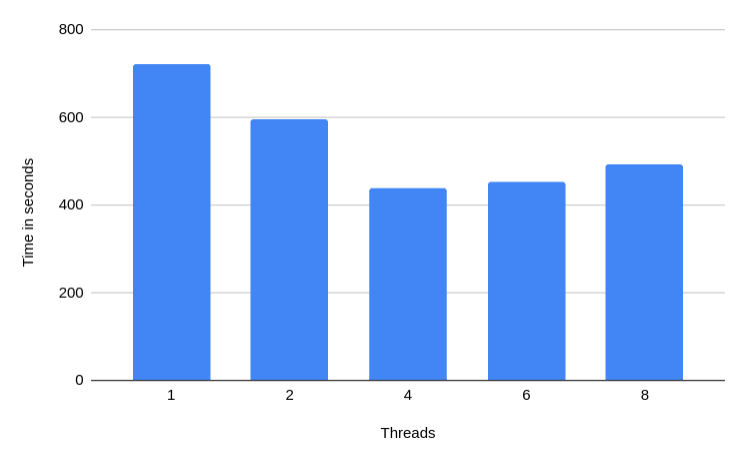
\includegraphics[width=13cm]{images/threads-table.png}
     \caption{Comparing threads performance.}
     \label{fig:threads-table}
\end{figure}


Another vital step in evaluating the effectiveness of multithreading is examining the distribution of shared links among threads. This is crucial to prevent one thread from overburdening while others remain idle, which would be inefficient, especially when using cloud services like AWS, where resources come at a cost. We'll perform this evaluation using the same configurations from Table \ref{table:crawler_test_config_depth_10}, employing four threads.

Figure \ref{fig:threads-share} displays the results of four runs, with each run showcasing a distinct distribution of crawled links among threads. While the ideal scenario would involve each thread handling 25\% of the discovered links, the averages in the columns reveal variations. Thread #4 crawls more than 25\%, while Thread #1 crawls less, which is normal due to considerations like communication overhead and thread-specific conditions. Additionally, threads won't split links if their queue contains fewer than five links, further affecting equal distribution.

\begin{figure}[H]	
     \centering
     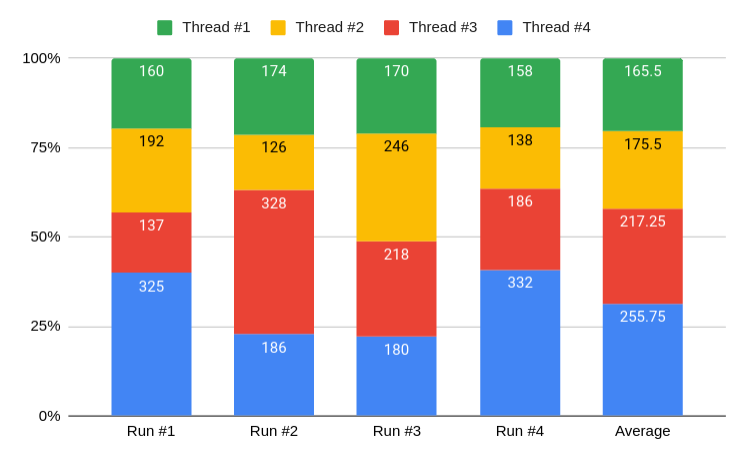
\includegraphics[width=13cm]{images/threads_share.png}
     \caption{Threads documents distribution.}
     \label{fig:threads-share}
\end{figure}


In order to assess the versatility of the web crawler and its adaptability to various usage scenarios, we will test three additional websites. The initial test case involves crawling a university ranking website to retrieve comprehensive information about all the universities listed, including their titles, respective countries, and current world rankings. The configuration parameters used for crawling this university-ranking website are detailed in Table \ref{table:crawler_conf_uni}.
To accommodate the structure of the website, where each page displays a table containing 25 universities, the "Allow Multi Element" flag is set to True. Considering the pagination feature on the website, which goes up to page 94, we have set the "Max Pages" parameter to 100, as it is unlikely that there will be more than 100 pages to crawl. Since we aim to extract three distinct pieces of information from the table, namely each university's Title, Location, and Ranking, we require three separate inspectors.
Given that each page comprises 25 universities, and there are 94 pages in total, we estimate a maximum of 2,350 documents to be collected during the crawling process.


\begin{table}[ht] 
{\footnotesize
\begin{tabular}{ P{3cm} ||P{10.1cm}  }      % centered columns (3 columns) 
 \hline \hline
\textbf{Seed URL} & \href{https://www.timeshighereducation.com/world-university-rankings/2023/world-ranking}{https://www.timeshighereducation.com/world-university-rankings/2023/world-ranking}\T\B 
\\ 
\hline
\textbf{Allow Multi Elements} & True \T\B 
\\ 
\hline
\textbf{Max Pages} & 100\T\B 
\\ 
\hline
\textbf{Threads} & 1\T\B 
\\ 
\hline
\textbf{Max Depth} & 100\T\B 
\\ 
\hline
\textbf{Pagination} & //*[contains(@class, 'pagination')]\T\B 
\\ 
\hline
\textbf{Actions} & None\T\B 
\\ 
\hline
\textbf{Inspectors} & //*[contains(@class, 'ranking-institution-title')] \newline //*[contains(concat(' ', normalize-space(@class), ' '), ' location ')] \newline //*[contains(@class, 'rank') and contains(@class, 'sorting\_1') and contains(@class, 'sorting\_2')]
\T\B 
\\ 
\hline
\textbf{Max Docs} & 2350\T\B 
\\ 
\hline \hline
    \end{tabular}
}
  \captionsetup{justification=centering,margin=2cm}
  \caption{Crawler configuration}
  \label{table:crawler_conf_uni}
\end{table}

The collected and visited links are accurate and match the expected count of 94. The fact that there are zero already visited links indicates that no duplicate URLs have been encountered. The total time spent during this process is approximately 8 minutes, which is significantly shorter compared to a similar test conducted using ParseHub, which took 20 minutes to complete all 94 pages.
Interestingly, even though the crawler successfully parsed and collected the results correctly, it consistently received a 403\footnote{The HTTP 403 Forbidden status code signifies that the server comprehends the request but declines to grant authorization for it.} status code in response to all HTTP requests instead of the expected 200. This issue may be attributed to the website's use of Cloudflare service, as suggested by the information available at ScrapeOps\footnote{\url{https://scrapeops.io/web-scraping-playbook/403-forbidden-error-web-scraping/}} .
In this particular use case, the number of collected documents representing universities in the table matches the total results displayed in the page pagination, totalling 2345. It is worth noting that the website also deploys a Robots.txt file, which the crawler successfully detected and used.

\begin{table}[ht] 
{\footnotesize
\begin{tabular}{ P{2.5cm} ||P{11.1cm}  }      % centered columns (3 columns) 
 \hline \hline
\textbf{Links} & 
\begin{tabular}{c|c|c|c|c}
       Collected   & Visited Correctly & Already Visited & Cross Site &  Excluded\T\B \\\hline
       94/94 & 94 & 0 & 0 & 0
\end{tabular}
\\ 
\hline
\textbf{Time} &
\begin{tabular}{P{3cm}|P{3cm}|P{3cm}}
       Tot. Spent & Avg. Processing & Avg. Page Rendering \T\B \\\hline
       351.66 s & 2.57 s & 1.020 s 
\end{tabular}
\\
\hline
\textbf{Status Codes} &  403: 94\T\B 
\\ 
\hline
\textbf{Docs \& Content} & 
\begin{tabular}{c|c|c|c}
       Tot. Docs   & Duplicated Content & Avg. Docs Per Page & Avg. Page Size\T\B \\\hline
       2345 & 0 & 25 & 0.2227
\end{tabular}
\\ 
\hline
\textbf{Robots.txt Exists} & True\T\B 
\\ 
\hline
\textbf{Tot. Errors} & 0\T\B 
\\ 
\hline \hline
    \end{tabular}
}
  \captionsetup{justification=centering,margin=2cm}
  \caption{Crawler configuration}
  \label{table:crawler_result_uni}
\end{table}


The following use case involves extracting a specific category of products from an e-commerce website. In this scenario, we will gather various types of data, including text and images. You can find the crawler configurations for this task in Table \ref{table:crawler_conf_douglas}, designed to scrape a particular product category.
Given that the Seed URL link's pagination indicates the presence of 7 pages, we can configure the Max Pages and Max Docs parameters to be 10. We can employ multithreading to increase performance by setting the number of threads to 4. Douglas employs lazy loading for image loading, which, in turn, causes the crawler to fetch only 30 out of the available 48 products on the page. To address this issue, we can utilize the actions tab to introduce a scrolling action, repeating it ten times until we reach the bottom of the page.
The ability to configure automated actions depends on the website's functionality. For instance, if the website experiences prolonged loading times, we can include a waiting action to account for the estimated waiting time. If the website necessitates a clicking action to reveal more information, the click action can be utilized for that purpose. The inspectors in this context encompass four fields: brand, title, price, and product images.


\begin{table}[ht] 
{\footnotesize
\begin{tabular}{ P{3cm} ||P{10.1cm}  }      % centered columns (3 columns) 
 \hline \hline
\textbf{Seed URL} & \href{https://www.douglas.de/de/c/parfum/damenduefte/duftsets/010111}{https://www.douglas.de/de/c/parfum/damenduefte/duftsets/010111}\T\B 
\\ 
\hline
\textbf{Allow Multi Elements} & True \T\B 
\\ 
\hline
\textbf{Max Pages} & 10\T\B 
\\ 
\hline
\textbf{Threads} & 4\T\B 
\\ 
\hline
\textbf{Max Depth} & 10\T\B 
\\ 
\hline
\textbf{Pagination} & //*[contains(@class, 'pagination')]\T\B 
\\ 
\hline
\textbf{Actions} & Scolling down 10 times\T\B 
\\ 
\hline
\textbf{Inspectors} & //*[contains(@class, 'top-brand')]\T\B  \newline
//a[contains(@class, 'product-tile\_\_main-link')]/div[1]/div/img \newline
//*[contains(@class, 'text')][contains(@class, 'name')] \newline
//div[contains(concat(' ', normalize-space(@class), ' '), ' price-row ')]\B  
\\ 
\hline
\textbf{Max Docs} & 1000\T\B 
\\ 
\hline \hline
    \end{tabular}
}
  \captionsetup{justification=centering,margin=2cm}
  \caption{Crawler configuration}
  \label{table:crawler_conf_douglas}
\end{table}

Table \ref{table:crawler_result_douglas} displays the outcomes obtained following the execution of the Douglas crawler. The "Collected" and "Visited" links align with the expected numbers within the targeted pagination. The estimated time taken for this operation is approximately 6.7 minutes. Notably, the "Average processing time" is more than double the time reported in the uni-ranking results in Table \ref{table:crawler_result_uni}. The primary reason for this extended processing time is the inclusion of additional scrolling-down actions.

It is noteworthy to consider an alternative approach: instead of scrolling down ten times to reach the page's end for image loading, why not employ a "scroll to the end of the page" event? This approach was tested on the Douglas website but proved ineffective. The reason is that specific frontend frameworks only load content when it is within the browser's view. Additionally, some websites, such as Facebook, initially display a limited number of posts on a user's home page, progressively loading more as the user scrolls down. In such cases, a single "jump to the end of the page" action will not suffice, as multiple scrolling-down actions are required.

The total count of collected documents indicates that 245 products were downloaded, which appears to be less than anticipated. Given that there are seven pages, with the first page containing 48 products, the theoretical result should be around 336 products. Further investigation revealed that only some pages contain exactly 48 products; some have more, while others have fewer.

It is important to note that, despite employing the robots.txt file for politeness and ensuring a relatively low crawler request rate (calculated as the number of threads divided by the Average Page Rendering, yielding 1.516 requests per second, which is relatively low and unlikely to overload the server), the IP address was eventually banned, and access to the site was blocked after several attempts. This highlights that each website may have its own unique security implementation based on its firewall\footnote{A firewall is a network security tool that filters and controls network traffic to safeguard against unauthorized access and cyber threats, serving as a barrier between trusted internal networks and untrusted external networks, such as the Internet.} rules and the reverse proxy\footnote{A reverse proxy is a server or software component that sits between client devices and a web server, forwarding client requests to the appropriate server and often providing additional functionalities like load balancing, caching, and security protection.} it uses.

Additionally, it's worth mentioning that the Douglas crawler was used without issue for three months, but a ban was encountered recently. This underscores that websites can adapt and modify their security measures over time.

\begin{table}[ht] 
{\footnotesize
\begin{tabular}{ P{2.5cm} ||P{11.1cm}  }      % centered columns (3 columns) 
 \hline \hline
\textbf{Links} & 
\begin{tabular}{c|c|c|c|c}
       Collected   & Visited Correctly & Already Visited & Cross Site &  Excluded\T\B \\\hline
       7/7 & 7 & 0 & 0 & 0
\end{tabular}
\\ 
\hline
\textbf{Time} &
\begin{tabular}{P{3cm}|P{3cm}|P{3cm}}
       Tot. Spent & Avg. Processing & Avg. Page Rendering \T\B \\\hline
       395.209 s & 7.87 s & 2.638 s 
\end{tabular}
\\
\hline
\textbf{Status Codes} & 200: 7\T\B 
\\ 
\hline
\textbf{Docs \& Content} & 
\begin{tabular}{c|c|c|c}
       Tot. Docs   & Duplicated Content & Avg. Docs Per Page & Avg. Page Size\T\B \\\hline
       245 & 0 & 49 & 1.509
\end{tabular}
\\ 
\hline
\textbf{Robots.txt Exists} & True\T\B 
\\ 
\hline
\textbf{Tot. Errors} & 0\T\B 
\\ 
\hline \hline
    \end{tabular}
}
  \captionsetup{justification=centering,margin=2cm}
  \caption{Crawler results}
  \label{table:crawler_result_douglas}
\end{table}


Parshub encountered a crash while running Douglas's project, resulting in the error message: "Segmentation fault (core dumped)." Although this made it challenging to compare performance, it shed light on Parsehub's stability issues, as Parsehub frequently struggles to handle websites without crashing.

Another use case involved crawling Stackoverflow questions, focusing solely on the "python" tag in the seed URL to retrieve Python-related questions. The configured inspectors collected question titles, descriptions, and vote counts. Initially, running the crawler with four threads led to a website ban after only ten pages were crawled. To resolve this, I reduced the thread count to one, reducing the number of requests and resolving the issue.


\begin{table}[ht] 
{\footnotesize
\begin{tabular}{ P{3cm} ||P{10.1cm}  }      % centered columns (3 columns) 
 \hline \hline
\textbf{Seed URL} & \href{https://stackoverflow.com/questions/tagged/python}{https://stackoverflow.com/questions/tagged/python}\T\B 
\\ 
\hline
\textbf{Allow Multi Elements} & True \T\B 
\\ 
\hline
\textbf{Max Pages} & 100\T\B 
\\ 
\hline
\textbf{Threads} & 1\T\B 
\\ 
\hline
\textbf{Max Depth} & 100\T\B 
\\ 
\hline
\textbf{Pagination} & //*[contains(@class, 's-pagination')]\T\B 
\\ 
\hline
\textbf{Actions} & None\T\B 
\\ 
\hline
\textbf{Inspectors} & //*[contains(@class, 's-post-summary--content-title')]\T\B  \newline
//*[contains(@class, 's-post-summary--content-excerpt')]	
 \newline
//*[contains(@class, 's-post-summary--stats-item\_\_emphasized')]	
\\ 
\hline
\textbf{Max Docs} & 1000\T\B 
\\ 
\hline \hline
    \end{tabular}
}
  \captionsetup{justification=centering,margin=2cm}
  \caption{Crawler configuration}
  \label{table:crawler_conf_stack}
\end{table}


Table \ref{table:crawler_result_stack} presents the crawler's results after this thread adjustment. Notably, the collected links exceeded those displayed in the pagination, indicating an issue with the pagination selector "s-pagination" collecting additional links. The number of visited pages reached 100, the configured limit, as intended, preventing the crawler from continuing to crawl all 27,200 found links. Many cross-site and excluded links signalled that the crawler had lost track and was collecting incorrect links. While 885 documents were collected correctly, there was no guarantee that they were all related to the chosen "Python" topic. Fortunately, termination conditions like Max Pages, Max Docs, and Max Depth were in place to conserve resources.

To troubleshoot the crawler, I enabled the 'Show Browser' option and reran it. This allowed for easier visualization of the crawler's behaviour and the links it was crawling. It revealed that the crawler was indeed lost and opening the wrong links. Despite the correct seed URL and pagination, the pagination selector 's-pagination' was missing from the configuration. This issue demonstrates how easy it is to debug and identify problems when a crawler loses its way, highlighting the crawler's politeness and stability.


\begin{table}[ht] 
{\footnotesize
\begin{tabular}{ P{2.5cm} ||P{11.1cm}  }      % centered columns (3 columns) 
 \hline \hline
\textbf{Links} & 
\begin{tabular}{c|c|c|c|c}
       Collected   & Visited Correctly & Already Visited & Cross Site &  Excluded\T\B \\\hline
       27200 & 100 & 0 & 460 & 666
\end{tabular}
\\ 
\hline
\textbf{Time} &
\begin{tabular}{P{3cm}|P{3cm}|P{3cm}}
       Tot. Spent & Avg. Processing & Avg. Page Rendering \T\B \\\hline
       588.505 s & 6.38 s & 0.561 s 
\end{tabular}
\\
\hline
\textbf{Status Codes} & 200: 99, 404:1 \T\B 
\\ 
\hline
\textbf{Docs \& Content} & 
\begin{tabular}{c|c|c|c}
       Tot. Docs   & Duplicated Content & Avg. Docs Per Page & Avg. Page Size\T\B \\\hline
       885 & 241 & 14 & 0.155
\end{tabular}
\\ 
\hline
\textbf{Robots.txt Exists} & True\T\B 
\\ 
\hline
\textbf{Tot. Errors} & 0\T\B 
\\ 
\hline \hline
    \end{tabular}
}
  \captionsetup{justification=centering,margin=2cm}
  \caption{Crawler results}
  \label{table:crawler_result_stack}
\end{table}

After fixing the second issue and rerunning the crawler, it operated correctly and yielded results in Table \ref{table:crawler_result_stack_2}. Notably, cross-site and excluded links were reduced to zero, a positive sign. Additionally, the number of collected links was lower than in the first attempt, totalling 900, with nine links collected per page. Interestingly, there were a significant number of 404 and 429 status codes. To address this, it could be beneficial to include a wait action between requests to mitigate the 429 errors.

When the same test was conducted using ParseHub, it took 20 minutes to complete, which was slower than the crawler's 6-minute runtime. It is worth noting that the two issues encountered during crawling were not experienced with ParseHub. This is because ParseHub's request rate is slower, reducing the risk of being banned. This is achieved by reducing the number of threads and can be further improved by adding wait actions. The second issue, concerning incorrect selectors, is where ParseHub shines as it offers an easy autodetect feature, simplifying selector selection with a simple click instead of manual XPATH insertion as required in the current crawler implementation.

\begin{table}[ht] 
{\footnotesize
\begin{tabular}{ P{2.5cm} ||P{11.1cm}  }      % centered columns (3 columns) 
 \hline \hline
\textbf{Links} & 
\begin{tabular}{c|c|c|c|c}
       Collected   & Visited Correctly & Already Visited & Cross Site &  Excluded\T\B \\\hline
       900 & 100 & 0 & 0 & 0
\end{tabular}
\\ 
\hline
\textbf{Time} &
\begin{tabular}{P{3cm}|P{3cm}|P{3cm}}
       Tot. Spent & Avg. Processing & Avg. Page Rendering \T\B \\\hline
       354.734 s & 2.66 s & 0.155 s 
\end{tabular}
\\
\hline
\textbf{Status Codes} & 200: 54, 404:21, 429: 25 \T\B 
\\ 
\hline
\textbf{Docs \& Content} & 
\begin{tabular}{c|c|c|c}
       Tot. Docs   & Duplicated Content & Avg. Docs Per Page & Avg. Page Size\T\B \\\hline
       2750 & 0 & 50 & 0.155
\end{tabular}
\\ 
\hline
\textbf{Robots.txt Exists} & True\T\B 
\\ 
\hline
\textbf{Tot. Errors} & 0\T\B 
\\ 
\hline \hline
    \end{tabular}
}
  \captionsetup{justification=centering,margin=2cm}
  \caption{Crawler results}
  \label{table:crawler_result_stack_2}
\end{table}

\section{Indexer}  

Following the initial crawling phase, the next step involves indexing, which requires a dedicated section for evaluation. To perform a thorough assessment of indexing, we will utilize a real-world dataset obtained through one of the crawlers employed during the evaluation process. We selected the Stack Overflow dataset presented in Table \ref{table:crawler_conf_stack} out of the three available use cases. The primary rationale for this choice is its larger size compared to the others, along with the presence of descriptions that can be employed for index evaluation. It is important to note that the crawler was rerun to gather additional Stack Overflow posts.

\subsection{Datasets}


\begin{table}[ht] 
{\footnotesize
\begin{tabular}{ P{3cm} ||P{10.1cm}  }      % centered columns (3 columns) 
 \hline \hline
\textbf{File Size} & 1.4MB \T\B 
\\ 
\hline
\textbf{Entries Count} & 2415\T\B 
\\ 
\hline
\textbf{Words Count} & 108122\T\B 
\\ 
\hline
\textbf{Fields} & Title, Summary, Votes\T\B 
\\ 
\hline \hline
    \end{tabular}
}
  \captionsetup{justification=centering,margin=2cm}
  \caption{Stack Overflow posts dataset}
    \label{table:indexer_dataset}
\end{table}

\subsection{Metrics}
We assess precision at a given value k (P@k), calculate the average precision (AP), and compute the normalized discounted cumulative gain at a specific position k (nDCG@k).

\subsection*{Precision at k (P@k)}
P@k represents the proportion of valid predictions within the system's top k predictions. We define $Q_{valid}$ as the collection of valid predictions for a question prefix q, as specified in the ground truth. Additionally, we denote $Q^k_{result}$ as the set of the system's top k completion predictions for a given question prefix q. The calculation for P@k is as follows:

\begin{equation}
P@k = \frac{|Q_{valid} \cap Q^k_{result}|}{k}
\label{eq:depth}
\end{equation}

We will compute the precision at 5 (p@5) for all the various indexing configurations.

\subsection*{Average Precision (AP)}
Consider $R_1$ through $R_k $ as the ordered list of positions where relevant documents are located within the result list of a specific query. In this context, Average Precision (AP) is computed as the mean of the k Precision at $R_i$ ($P@R_i$) values. AP is computed as:

\begin{equation}
AP = \frac{\sum_{i=1}^{n} P@r_i}{n}
\label{eq:depth}
\end{equation}

For the predictions from $Q_{valid}$ that are absent in $Q_{result}$, we assign a Precision at position $r_i $ (P@ri) value of 0. We then calculate the average precision by averaging these values across all question prefixes in the ground truth.

\subsection*{Mean Precisions (MP@k, MP@R, MAP)}
Having a benchmark containing multiple queries and their corresponding ground truth data, we can assess the system's performance by calculating the average value of a specific metric across all the queries.

MP@k represents the mean precision at k values across all queries, MP@R represents the mean precisionat R values across all queries, and MAP signifies the mean average precision values across all queries.

\subsection{Experiments}
 
 To assess the performance of our indexing, we will employ the Stack Overflow dataset listed in Table \ref{table:indexer_dataset}. We will modify the indexing attributes' settings and examine how these changes impact the evaluation metrics.
 
 We will initiate our indexing process using the default settings specified in Table \ref{table:indexer_conf_1}. The Stack Overflow dataset consists of three inspector fields: Title, Summary, and Votes. However, we intend to index only the textual fields, such as Title and Summary, while retaining Votes as they contain numerical data intended solely for ranking purposes. All other configuration parameters are set to their default values. For a clearer understanding of the configuration attributes, please refer to Table \ref{table:indexing-config}, which provides descriptions of each attribute.
 


\begin{table}[ht] 
{\footnotesize
\begin{tabular}{ P{3cm} ||P{10.1cm} }      % centered columns (3 columns) 
 \hline \hline
\textbf{Inspectors} & Title, Summary \T\B 
\\ 
\hline
\textbf{BM25 Parameters} & B=0.75, K=1.75\T\B 
\\ 
\hline
\textbf{Stop Words} & None\T\B 
\\ 
\hline
\textbf{Small Words Threshold} & 2\T\B 
\\ 
\hline
\textbf{Q-gram} & 3\T\B 
\\ 
\hline
\textbf{Boosting Formula} & None\T\B 
\\ 
\hline
\textbf{Result} & 
\begin{tabular}{P{2cm}|P{2cm}|P{2cm}|P{2cm}}
       \textbf{MP@5} & \textbf{MP@R} & \textbf{MAP} & \textbf{Time(s)}\T\B \\\hline
       0.73 & 0.72 & 0.87 & 0.31
\end{tabular}
\\
\hline \hline
    \end{tabular}
}
  \captionsetup{justification=centering,margin=2cm}
  \caption{Stack Overflow indexing configuration, test the default settings without any changes.}
      \label{table:indexer_conf_1}
\end{table}

Upon initiating the indexing process for the first time, without the availability of any caching, it may take up to two minutes to complete. This indexing procedure consists of two distinct stages: the first involves the creation of a dictionary, which aids in providing suggestions in the dropdown menu to help users locate the appropriate queries. Creating this dictionary is the longer of the two stages, typically taking around 1.8 minutes, while the indexing phase takes approximately seven seconds. The primary disparity between these stages lies in the size of the entities involved; the dictionary comprises 2.6 million entities, whereas the Stack Overflow entities used for indexing consist of only two thousand entities. It is worth noting that the overall duration of the indexing process is highly contingent on the size of the file being indexed and, in this case, the volume of documents crawled by the web crawler. Following the initial indexing process, the dictionary index will be cached and no longer require further indexing.

Even though the search results return 25 documents, we will set the value of k for the P@k metric to 5. This choice is based on the everyday user preference for focusing on the top results in a search list. The overall metrics are presented in Table \ref{table:indexer_conf_1}. While these results indicate reasonable accuracy, it is essential to acknowledge that assessing relevance can be subjective, as it varies among users. For instance, Google's ranking system considers factors like user location, link authenticity, and text matching, leading to potentially inconsistent results for the same query across different users.
Furthermore, aiming for an extremely high level of accuracy can lead to model overfitting\footnote{Overfitting in data science happens when a model fits its training data too closely. This leads to poor performance when dealing with new, unseen data.}, causing it to struggle with generalization. While it may achieve a high precision score with benchmark data, it may need to improve when faced with new, unseen queries. This is because all the model's parameters have been fine-tuned to fit the benchmark datasets perfectly. Therefore, balancing achieving a reasonable precision score and ensuring that the model performs well on new, previously unseen datasets is crucial. Therefore, achieving perfect accuracy scores in evaluations is challenging and involves a trade-off. The Precision@K metric is significantly affected by the selection of both the value of K and the relevance threshold. Different choices for K and the threshold can result in varying Precision@K scores for the same model. As a result, it is essential to carefully and consistently choose these parameters when comparing different models.

\begin{table}[ht] 
{\footnotesize
\begin{tabular}{ P{3cm} ||P{10.1cm}  }      % centered columns (3 columns) 
 \hline \hline
\textbf{Inspectors} & Title, Summary \T\B 
\\ 
\hline
\textbf{BM25 Parameters} & B=0.1, K=0.81\T\B 
\\ 
\hline
\textbf{Stop Words} & None\T\B 
\\ 
\hline
\textbf{Small Words Threshold} & 2\T\B 
\\ 
\hline
\textbf{Q-gram} & 3\T\B 
\\ 
\hline
\textbf{Boosting Formula} & None\T\B 
\\ 
\hline
\textbf{Result} & 
\begin{tabular}{P{2cm}|P{2cm}|P{2cm}|P{2cm}}
       \textbf{MP@5} & \textbf{MP@R} & \textbf{MAP} & \textbf{Time(s)}\T\B \\\hline
       0.8 & 0.84 & 0.89 & 0.31
\end{tabular}
\\
\hline \hline
    \end{tabular}
}
  \captionsetup{justification=centering,margin=2cm}
  \caption{Stack Overflow indexing configuration}
  \label{table:indexer_conf_2}
\end{table}

The initial parameters to adjust are b and k. Table \ref{table:indexer_conf_2} displays the configuration of the Stack Overflow indexer, with modifications made to the default b and k values. These values have increased. The key takeaway is that modifying the attributes available in the indexing user interface can enhance or diminish accuracy, providing users with a convenient way to fine-tune their model.

\begin{table}[ht] 
{\footnotesize
\begin{tabular}{ P{3cm} ||P{10.1cm}  }      % centered columns (3 columns) 
 \hline \hline
\textbf{Inspectors} & Title, Summary \T\B 
\\ 
\hline
\textbf{BM25 Parameters} & B=0.1, K=0.81\T\B 
\\ 
\hline
\textbf{Stop Words} & how, to, by, with, in, not, does\T\B 
\\ 
\hline
\textbf{Small Words Threshold} & 2\T\B 
\\ 
\hline
\textbf{Q-gram} & 3\T\B 
\\ 
\hline
\textbf{Boosting Formula} & None\T\B 
\\ 
\hline
\textbf{Result} & 
\begin{tabular}{P{2cm}|P{2cm}|P{2cm}|P{2cm}}
       \textbf{MP@5} & \textbf{MP@R} & \textbf{MAP} & \textbf{Time(s)}\T\B \\\hline
       0.66 & 0.624 & 0.76 & 0.31
\end{tabular}
\\
\hline \hline
    \end{tabular}
}
  \captionsetup{justification=centering,margin=2cm}
  \caption{Stack Overflow indexing configuration}
    \label{table:indexer_conf_3}
\end{table}


Let us retain the modified b and k parameters instead of using the default values, as they produce improved results. The following attribute we consider for indexing includes stop words and examining their impact on accuracy. Initially, the intuition is to remove common words such as "how," "to," "by," "with," "in," "not," and "does" from the benchmark queries since they may seem insignificant and lack essential information. Surprisingly, though, removing these words leads to a reduction in accuracy as illustraded in Table \ref{table:indexer_conf_3}.

This could be attributed to the Stack Overflow dataset not being exceptionally large, and the assumption that these words are common in the English language may not hold for some queries in the small Stack Overflow dataset. Furthermore, stop words are not just about eliminating common words; they can also be used to consistently disregard words that typically provide no meaningful information in a query. For example, in the current Stack Overflow dataset, which encompasses all posts related to Python, including the term "python" in the query should have no impact, as all the posts are Python-related, even if they do not explicitly mention the word "python" but discuss Python libraries, for instance.

It is important to note that stop words containing two characters or fewer have no impact in this context and can be safely eliminated. The rationale is that they should already be filtered out due to the Small Words Threshold being set to two.


\begin{table}[ht] 
{\footnotesize
\begin{tabular}{ P{3cm} ||P{10.1cm}  }      % centered columns (3 columns) 
 \hline \hline
\textbf{Inspectors} & Title, Summary \T\B 
\\ 
\hline
\textbf{BM25 Parameters} & B=0.1, K=0.81\T\B 
\\ 
\hline
\textbf{Stop Words} & None\T\B 
\\ 
\hline
\textbf{Small Words Threshold} & 0\T\B 
\\ 
\hline
\textbf{Q-gram} & 3\T\B 
\\ 
\hline
\textbf{Boosting Formula} & None\T\B 
\\ 
\hline
\textbf{Result} & 
\begin{tabular}{P{2cm}|P{2cm}|P{2cm}|P{2cm}}
       \textbf{MP@5} & \textbf{MP@R} & \textbf{MAP} & \textbf{Time(s)}\T\B \\\hline
       0.8 & 0.77 & 0.84 & 0.31
\end{tabular}
\\
\hline \hline
    \end{tabular}
}
  \captionsetup{justification=centering,margin=2cm}
  \caption{Stack Overflow indexing configuration}
  \label{table:indexer_conf_4}
\end{table}

In the following evaluation in Table \ref{table:indexer_conf_4}, we adjust the Small Words Threshold to zero, which implies that no words are excluded during the indexing process. While the results remain reasonably good, there has been a decrease in precision. This suggests that in certain cases, increasing the Small Words Threshold and not setting it to zero may be advisable. However, it's essential to exercise caution when eliminating small words, particularly those with one to three characters, depending on the language. Additionally, it's worth noting that some two-character words can be acronyms, such as "OS" (Operating System).

\begin{table}[ht] 
{\footnotesize
\begin{tabular}{ P{3cm} ||P{10.1cm}  }      % centered columns (3 columns) 
 \hline \hline
\textbf{Inspectors} & Title, Summary \T\B 
\\ 
\hline
\textbf{BM25 Parameters} & B=0.1, K=0.81\T\B 
\\ 
\hline
\textbf{Stop Words} & None\T\B 
\\ 
\hline
\textbf{Small Words Threshold} & 2\T\B 
\\ 
\hline
\textbf{Q-gram} & 3\T\B 
\\ 
\hline
\textbf{Boosting Formula} & $\frac{votes}{10}$\T\B 
\\ 
\hline
\textbf{Result} & 
\begin{tabular}{P{2cm}|P{2cm}|P{2cm}|P{2cm}}
       \textbf{MP@5} & \textbf{MP@R} & \textbf{MAP} & \textbf{Time(s)}\T\B \\\hline
       0.53 & 0.62 & 0.63 & 0.31
\end{tabular}
\\
\hline \hline
    \end{tabular}
}
  \captionsetup{justification=centering,margin=2cm}
  \caption{Stack Overflow indexing configuration}
  \label{table:indexer_conf_5}
\end{table}

The final attribute to adjust is the Boosting Formula. The Boosting Formula is an optional field and particularly useful for ranking documents containing a numeric field. Examples of such fields include product prices, product reviews, post likes, post shares, or the order of items in a list, like the example of university rankings.
In the specific context of the Stack Overflow example, each post is associated with an upvote number, which indicates how helpful an answer is. This numeric field can be a valuable indicator of document quality and relevance. The more users find a post helpful, the more valuable it becomes to display it as one of the top results. To assign a higher score to posts with a high number of votes, we can employ the Boosting Formula. One practical choice is to use the logarithm of the votes. However, since votes can be zero or even negative, more suitable options may exist. We will utilize the formula shown in \ref{table:indexer_conf_5} for this straightforward use case.


\section{User Experience} 

Throughout this project, I had the opportunity to work with ParseHub software. While this experience does not make me an expert, I did gain practical knowledge in using ParseHub for various aspects of web crawling, which proved beneficial for the thesis. There are notable advantages and disadvantages when comparing ParseHub with the current implementation used in the thesis.

One of the standout features of ParseHub is its automatic detection of document fields, achieved by clicking. In contrast, my implementation requires manual input of HTML element XPATH to obtain this information. Creating the crawlers manually in my implementation often took more than ten minutes, whereas ParseHub accomplished the same results in half the time. Another advantage of ParseHub is its project-based approach to crawling, as opposed to my implementation's list of crawlers. Starting a crawler in ParseHub can be done by providing only the Seed URL without further options, simplifying the process. However, it is essential to note that this feature can be easily extended and is a manageable hurdle.

In terms of performance, the current implementation excels, as demonstrated in the evaluation tables. Additionally, the current implementation allows for the addition of more threads and nodes to enhance performance, a flexibility not available in ParseHub. Furthermore, the current implementation has proven resilient in handling various edge cases, whereas ParseHub struggled to manage these scenarios effectively. The adaptability and configuration options offered by the current implementation make it well-suited for various websites and scenarios.

The user interface employed in ParseHub needs to be updated; it lacks responsiveness and features a font that is challenging to read. However, the most frustrating aspect is the frequent occurrence of the browser unexpectedly crashing and shutting down without apparent cause. In contrast, utilizing a frontend framework like Angular with PrimeNG significantly improved the current implementation, making it responsive and delivering a seamless user experience.

One notable drawback of ParseHub is its need for indexing capabilities. When crawling a large dataset, having an indexed version of the data becomes crucial, mainly if the dataset is intended to be served as an API, for example.